\section{Aufbau eines regelbasierten Wissensbasierten Systems}

Regelbasierte Systeme basieren auf dem Prinzip eines Produktionssystems zur Termersetzung (Emil Post 1943). Eine �bersicht �ber ein komplettes Produktionssystems ist in Abbildung~\ref{fig:xps-overview} dargestellt.

\begin{figure}[H]
    \centering
    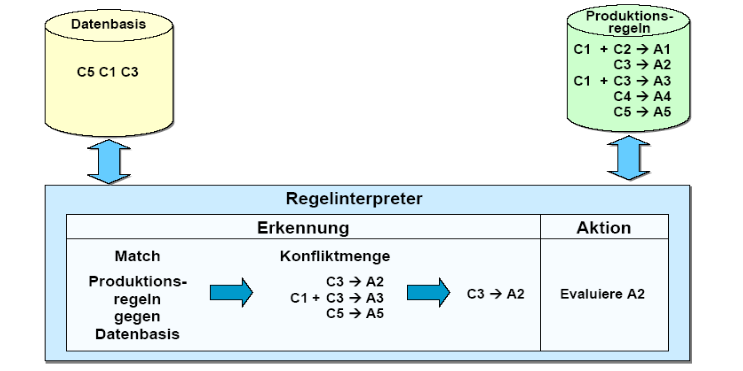
\includegraphics[width=0.9\textwidth]{figures/kap7/overview-xps.png}
    \caption{Produktionssystems zur Termersetzung}
    \label{fig:xps-overview}
\end{figure}

Eine Produktion, auch als ``Regel'' bekannt, besteht aus zwei Teilen (Abb.~\ref{fig:xps-regelstruktur}).

\begin{figure}[H]
    \centering
    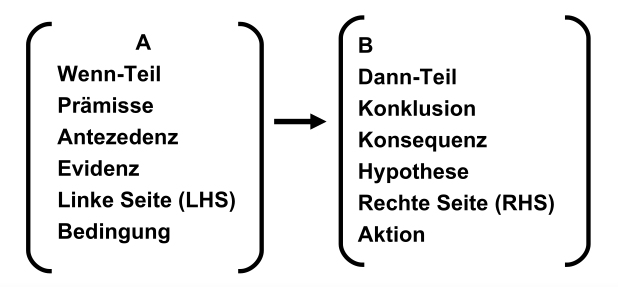
\includegraphics[width=0.8\textwidth]{figures/kap7/production-system-parts.png}
    \caption{Regelstruktur eines regelbasierten Expertensystems}
    \label{fig:xps-regelstruktur}
\end{figure}

Grunds�tzlich basieren die Regeln auf einer Kombination der Teile von A und Teilen von B. Zum Beispiel: Wenn A1 und A2 und An, \textbf{dann} B1 und B2 und Bn und Bm und so weiter. 

Anhand dieser Regeln kann Wissen von Experten gebildet werden. Tats�chlich arbeiten viele Expertensysteme mit einer einfachen Form von IF <Begingung> THEN <Konsequenz>.